\section{Calibration}
\begin{frame}{Calibration MVA variables}
  \begin{itemize}
  \item E\(_{\text{acc}}\) : sum of uncalibrated energies measured in the accordion.
  \item E\(_{\text{0}}\)/E\(_{\text{acc}}\) : ratio of the energy in the presampler over the energy in the accordion.
  \item $E_1/E_2$ : ratio of the uncalibrated energy in the first over the second layer ($E_1/E_2$).
  \item \(\eta_{\text{cluster}}\) :  pseudo rapidity in the ATLAS frame.
  \item Cell index : an integer number defined as the integer part of the division ( \(\eta_{\text{calo}}\)/\(\Delta \eta\)) where \(\eta_{\text{calo}}\) is the cluster pseudo rapidity in the calorimeter frame with \(\Delta \eta\) as the size of one cell in the middle layer. 
  \item $\eta$ position of the cluster with respect to the cell edge.
  \item $\phi$ with respect to the lead absorber. This variable is sensitive to the modulation of the thickness of the absorber as a function of $\phi$.
  \end{itemize}
\end{frame}

%====================================
\begin{frame}{Template method}
  \begin{minipage}{0.59\linewidth}
    Minimum of $\chi^2$ distribution fitted in 2 steps of 1D fits : 
    \begin{itemize}
    \item \textcolor{red}{fit $\chi^2=f(\alpha)$ at constant $c$ (lines)} $\rightarrow (\alpha_{min}, \chi^2_{min})$ .
    \item \textcolor{blue}{fit $\chi^2_{min}=f(c)\rightarrow (c, \Delta c)$}
    \item \textcolor{brown}{project $c$ in $\alpha_{min}=f(c)$}, corresponding bin gives $(\alpha, \Delta\alpha)$.
    \end{itemize}
  \end{minipage}
\hfill
\begin{minipage}{0.4\linewidth}
%  \includegraphics[width=\linewidth]{MC6_0_0_CompareAlpha.pdf}\\
  \includegraphics[width=\linewidth]{MC6_0_0_chiMatrix.pdf}\\
\end{minipage}
    \begin{tikzpicture}
      \node[anchor=south west] {
        \includegraphics[width=0.325\linewidth]{MC6_0_0_chi2FitNonConstVar_10.pdf}
        \includegraphics[width=0.325\linewidth]{MC6_0_0_chi2FitConstVar.pdf}
        \includegraphics[width=0.325\linewidth]{MC6_0_0_corAngle.pdf}
      };
%      \draw[step=1.0,black,thin] (0,0) grid (10,3);
      \draw[red, line width=0.5mm, rounded corners =2pt] ( 0.1, 0.05 ) rectangle ( 4.03, 3 ) ;
      \draw[blue, line width=0.5mm, rounded corners =2pt] ( 4.03, 0.05 ) rectangle ( 7.95, 3 ) ;
      \draw[brown, line width=0.5mm, rounded corners =2pt] ( 7.95, 0.05 ) rectangle ( 12, 3 ) ;
      \end{tikzpicture}


\end{frame}

%====================================
\begin{frame}{In situ calibration $\eta_\text{calo}$ bin frontiers}
        {\tiny \textcolor{brown}{0} 0.1 \textcolor{brown}{0.2} 0.3 \textcolor{brown}{0.4} 0.5 \textcolor{brown}{0.6} 0.7 \textcolor{brown}{0.8} 0.9 \textcolor{brown}{1} 1.1 \textcolor{brown}{1.2} 1.285 \textcolor{brown}{1.37} 1.42 1.47 1.51 \textcolor{brown}{1.55} 1.59 1.63 1.6775 1.725 1.7625 \textcolor{brown}{1.8} 1.9 \textcolor{brown}{2} 2.05 2.1 2.2 \textcolor{brown}{2.3} 2.35 2.4 2.435 \textcolor{brown}{2.47}}
\end{frame}

%===============================================
\begin{frame}{In-situ 2015 pre-recommandations : binning uncertainty}
  \centering
  \includegraphics[width=0.9\linewidth]{/home/goudet/Documents/LAL/Zim/Calibration/PreRec/150727_ComparisonBins_alpha.png}
  \end{frame}
%===============================================
\begin{frame}{In situ scale uncertainties uncertainties}
  12 (13) sources of uncertainties have been evaluated for $\alpha$ ($c$).

    \begin{minipage}{0.49\linewidth} 
      \includegraphics[width=\linewidth]{CalibSupNote_totUncAlpha.pdf}
  \end{minipage}
  \hfill
  \begin{minipage}{0.49\linewidth}
    \includegraphics[width=\linewidth]{CalibSupNote_totUncC.pdf}
  \end{minipage}

\end{frame}

%===========================================
\begin{frame}{Photon correction}
Electrons scale factors are also applied to photons. 
A residual scale factor ($\Delta\alpha$) is measured from $Z\rightarrow ll\gamma$.

No significant deviation observed.
\newline
  \begin{minipage}{0.49\linewidth}
    \includegraphics[width=\linewidth]{CERN-PH-EP-2014-153_34fa.pdf}
  \end{minipage}
  \hfill
  \begin{minipage}{0.49\linewidth}
    \includegraphics[width=\linewidth]{CERN-PH-EP-2014-153_34fb.pdf}
  \end{minipage}
\end{frame}

%============================================

\section{In situ Technicalities}



\begin{frame}{$c$ fit }
  $$ a_0(c)=b_0+\frac{(c-\hat{c})^2}{\textcolor{red}{b_2}^2} + b_1 . \frac{(c-\hat{c})^3}{\textcolor{red}{b_2}^3}$$
  
  \begin{minipage}{0.49\linewidth}
    \includegraphics[width=\linewidth]{/home/goudet/Documents/LAL/Zim/Calibration/TemplateMethod/151028_DichotomyErr.pdf}
  \end{minipage}
  \hfill
  \begin{minipage}{0.49\linewidth}
    \begin{equation}
      \textcolor{blue}{P( \hat{c} + \delta c) = 1}
    \end{equation}
    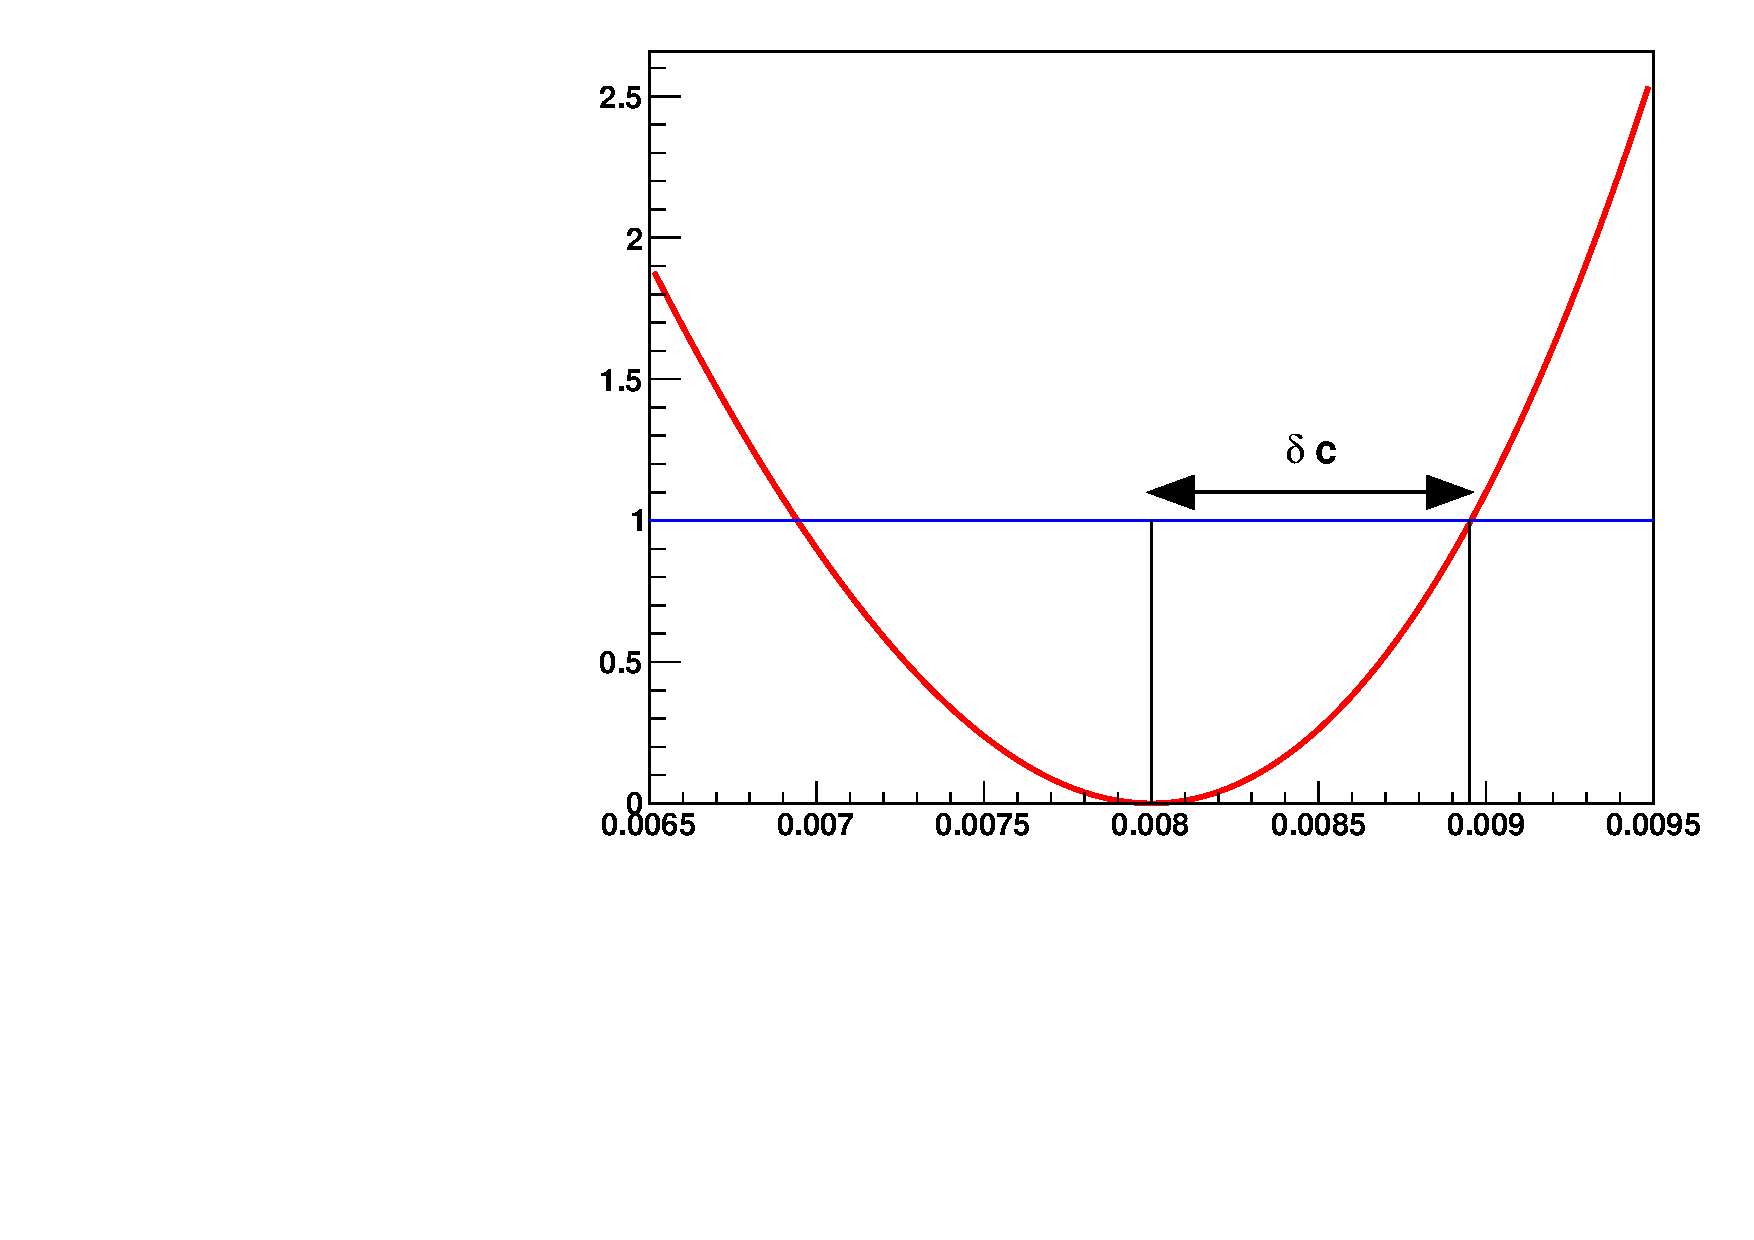
\includegraphics[width=\linewidth]{Figures/pol3.pdf}
\end{minipage}
\end{frame}

%=============================================
\begin{frame}{Z mass distribution binning}
\begin{figure}
\begin{subfigure}[t]{0.49\linewidth}
\begin{center}
\includegraphics[width=\linewidth]{/home/goudet/Documents/LAL/Zim/Calibration/TemplateMethod/PlotsIllustration/Closure_0_0.pdf}
\end{center}
\caption{20 bins}
\end{subfigure}
\begin{subfigure}[t]{0.49\linewidth}
\begin{center}
\includegraphics[width=\linewidth]{/home/goudet/Documents/LAL/Zim/Calibration/TemplateMethod/PlotsIllustration/Closure_0_0_40MassBin.pdf}
\end{center}
\caption{40 bins}
\end{subfigure}
\caption{\label{org955c893}
Comparison of $\chi^2$ distributions for different Z mass distribution binnings.}
\end{figure}
  \end{frame}

%======================================
\begin{frame}{Scale range optimisation}
  \begin{minipage}{0.49\linewidth}
      \includegraphics[width=\linewidth]{Closure_0_0_noOptim.pdf}
  \end{minipage}
  \hfill
  \begin{minipage}{0.49\linewidth}
      \includegraphics[width=\linewidth]{Closure_0_0_1Optim.pdf}
  \end{minipage}
  \begin{minipage}{0.49\linewidth}
      \includegraphics[width=\linewidth]{Closure_0_0.pdf}
  \end{minipage}
  \hfill
  \begin{minipage}{0.49\linewidth}
    \begin{itemize}
    \item top left : arbitrary conservative values
    \item top right : $1\sigma$ range
    \item bottom left : $5\sigma$
    \end{itemize}
  \end{minipage}
\end{frame}
%=============================================
\begin{frame}{Template correlation}
  \begin{figure}
\begin{subfigure}[t]{0.49\linewidth}
\begin{center}
\includegraphics[width=\linewidth]{Closure_0_0.pdf}
\end{center}
\caption{correlated}
\end{subfigure}
\begin{subfigure}[t]{0.49\linewidth}
\begin{center}
\includegraphics[width=\linewidth]{Closure_0_0_uncorTemp.pdf}
\end{center}
\caption{uncorrelated}
\end{subfigure}
\caption{\label{orgff6a45b}
Comparison of $\chi^2$ distribution between a correlated and uncorrelated MC template smearing. Uncorrelated supposes that mass smearings in two different templates use different random numbers.}
\end{figure}
\end{frame}

%========================================
\begin{frame}{$N_\text{useEl}$}
  \begin{figure}
\begin{subfigure}[t]{0.49\linewidth}
\begin{center}
\includegraphics[width=\linewidth]{Closure_0_0.pdf}
\end{center}
\caption{$N_\text{useEl}=1$}
\end{subfigure}
\begin{subfigure}[t]{0.49\linewidth}
\begin{center}
\includegraphics[width=\linewidth]{Closure_0_0_10nUseEl.pdf}
\end{center}
\caption{$N_\text{useEl}=10$}
\end{subfigure}
\caption{\label{org98e07ca}
$\chi^2$ distribution for a typical configuration for different values of $N_\text{useEl}$. In both cases, pseudo-data corresponds to the same dataset as the MC in which a constant term has been injected.}
\end{figure}
\end{frame}

%==========================================
\begin{frame}{Inversion}
  \centering
\textcolor{blue}{  fitC : $\chi_c^2 = \sum \limits_{i, j\leq i} \frac{ (\sqrt{\frac{c_i^2 + c_j^2}{2}} - c_{ij})^2 }{(\delta c_{ij})^2}$ } \\

  \textcolor{purple}{fitC2 : $\chi_{c2}^2 = \sum \limits_{i, j\leq i} \frac{ (\frac{c_i^2 + c_j^2}{2} - c_{ij}^2)^2 }{(\delta c_{ij}^2)^2}$}

  \begin{figure}
\begin{subfigure}[t]{0.49\linewidth}
\begin{center}
\includegraphics[width=\linewidth]{/home/goudet/Documents/LAL/Zim/Calibration/TemplateMethod/150828_InversionStudy_Note.png}
\end{center}
\end{subfigure}
\begin{subfigure}[t]{0.49\linewidth}
\begin{center}
\includegraphics[width=\linewidth]{/home/goudet/Documents/LAL/Zim/Calibration/TemplateMethod/150828_InversionStudy_crossCheck.png}
\end{center}
\end{subfigure}
\caption{\label{orgac9241c}
Comparison of closures for different inversion procedures.}
\end{figure}
\end{frame}
